\documentclass[tikz,border=10pt]{standalone}
\usepackage{tikz}
\usetikzlibrary{positioning, calc, arrows.meta, shapes.misc}

\begin{document}
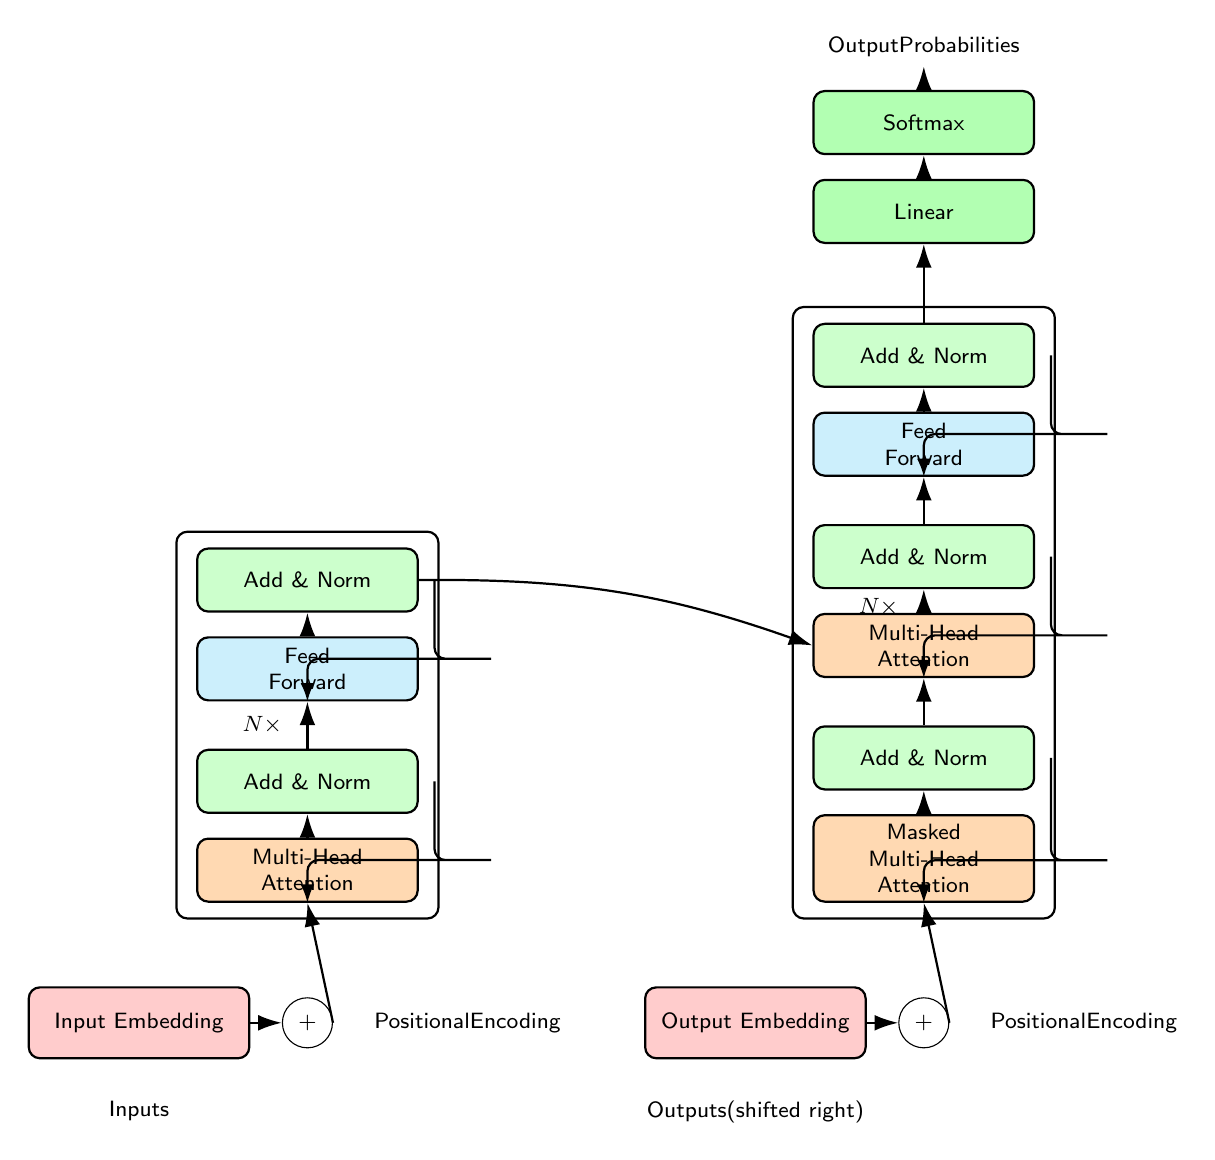
\begin{tikzpicture}[
  font=\sffamily,
  >=Latex,
  box/.style={rectangle, draw, rounded corners, thick, align=center, minimum width=2.8cm, minimum height=0.9cm},
  smallbox/.style={rectangle, draw, rounded corners, thick, align=center, minimum width=2.8cm, minimum height=0.8cm},
  arrow/.style={-{Latex[length=3mm, width=2mm]}, thick},
  addnorm/.style={fill=green!20},
  attn/.style={fill=orange!30},
  ffn/.style={fill=cyan!20},
  embed/.style={fill=red!20},
  output/.style={fill=green!30},
  every node/.style={font=\sffamily\footnotesize}
]

%------------------------------------------------
% Encoder
%------------------------------------------------
\node[box, embed] (enc_embed) {Input Embedding};
\node[circle, draw, minimum size=0.5cm, right=0.4cm of enc_embed] (enc_add) {+};
\node[right=0.4cm of enc_add] (enc_pos) {Positional\\Encoding};

% Encoder layers
\node[smallbox, attn, above=1.2cm of enc_add] (enc_attn) {Multi-Head\\Attention};
\node[smallbox, addnorm, above=0.3cm of enc_attn] (enc_addnorm1) {Add \& Norm};
\node[smallbox, ffn, above=0.6cm of enc_addnorm1] (enc_ffn) {Feed\\Forward};
\node[smallbox, addnorm, above=0.3cm of enc_ffn] (enc_addnorm2) {Add \& Norm};

% Bracket and Nx label
\draw[thick, rounded corners] ($(enc_attn.south west)+(-0.25,-0.2)$) rectangle ($(enc_addnorm2.north east)+(0.25,0.2)$);
\node[left=0.2cm of $(enc_addnorm2)!0.5!(enc_attn)$] {$N\times$};

% Encoder arrows
\draw[arrow] (enc_embed.east) -- (enc_add.west);
\draw[arrow] (enc_add.east) -- (enc_attn.south);
\draw[arrow] (enc_attn.north) -- (enc_addnorm1.south);
\draw[arrow] (enc_addnorm1.north) -- (enc_ffn.south);
\draw[arrow] (enc_ffn.north) -- (enc_addnorm2.south);

%------------------------------------------------
% Decoder
%------------------------------------------------
\node[box, embed, right=5cm of enc_embed] (dec_embed) {Output Embedding};
\node[circle, draw, minimum size=0.5cm, right=0.4cm of dec_embed] (dec_add) {+};
\node[right=0.4cm of dec_add] (dec_pos) {Positional\\Encoding};

\node[smallbox, attn, above=1.2cm of dec_add] (dec_selfattn) {Masked\\Multi-Head\\Attention};
\node[smallbox, addnorm, above=0.3cm of dec_selfattn] (dec_addnorm1) {Add \& Norm};
\node[smallbox, attn, above=0.6cm of dec_addnorm1] (dec_crossattn) {Multi-Head\\Attention};
\node[smallbox, addnorm, above=0.3cm of dec_crossattn] (dec_addnorm2) {Add \& Norm};
\node[smallbox, ffn, above=0.6cm of dec_addnorm2] (dec_ffn) {Feed\\Forward};
\node[smallbox, addnorm, above=0.3cm of dec_ffn] (dec_addnorm3) {Add \& Norm};

% Bracket and Nx label
\draw[thick, rounded corners] ($(dec_selfattn.south west)+(-0.25,-0.2)$) rectangle ($(dec_addnorm3.north east)+(0.25,0.2)$);
\node[left=0.2cm of $(dec_addnorm3)!0.5!(dec_selfattn)$] {$N\times$};

% Decoder arrows
\draw[arrow] (dec_embed.east) -- (dec_add.west);
\draw[arrow] (dec_add.east) -- (dec_selfattn.south);
\draw[arrow] (dec_selfattn.north) -- (dec_addnorm1.south);
\draw[arrow] (dec_addnorm1.north) -- (dec_crossattn.south);
\draw[arrow] (dec_crossattn.north) -- (dec_addnorm2.south);
\draw[arrow] (dec_addnorm2.north) -- (dec_ffn.south);
\draw[arrow] (dec_ffn.north) -- (dec_addnorm3.south);

%------------------------------------------------
% Encoder-Decoder connection
%------------------------------------------------
\draw[arrow, bend left=10] (enc_addnorm2.east) to (dec_crossattn.west);

%------------------------------------------------
% Output layer
%------------------------------------------------
\node[smallbox, output, above=1cm of dec_addnorm3] (linear) {Linear};
\node[smallbox, output, above=0.3cm of linear] (softmax) {Softmax};
\node[above=0.3cm of softmax] (outlabel) {Output\\Probabilities};

\draw[arrow] (dec_addnorm3.north) -- (linear.south);
\draw[arrow] (linear.north) -- (softmax.south);
\draw[arrow] (softmax.north) -- (outlabel.south);

%------------------------------------------------
% Input/Output labels
%------------------------------------------------
\node[below=0.4cm of enc_embed] {Inputs};
\node[below=0.4cm of dec_embed] {Outputs\\(shifted right)};

%------------------------------------------------
% Curved residual arrows (within encoder & decoder)
%------------------------------------------------
\draw[->, thick, rounded corners] ($(enc_addnorm1.east)+(0.2,0)$) |- ++(0.8,-1.0) -| ($(enc_attn.south)+(0,0)$);
\draw[->, thick, rounded corners] ($(enc_addnorm2.east)+(0.2,0)$) |- ++(0.8,-1.0) -| ($(enc_ffn.south)+(0,0)$);

\draw[->, thick, rounded corners] ($(dec_addnorm1.east)+(0.2,0)$) |- ++(0.8,-1.3) -| ($(dec_selfattn.south)+(0,0)$);
\draw[->, thick, rounded corners] ($(dec_addnorm2.east)+(0.2,0)$) |- ++(0.8,-1.0) -| ($(dec_crossattn.south)+(0,0)$);
\draw[->, thick, rounded corners] ($(dec_addnorm3.east)+(0.2,0)$) |- ++(0.8,-1.0) -| ($(dec_ffn.south)+(0,0)$);

\end{tikzpicture}
\end{document}

